\subsection{Structures}
\subsubsection{Material Selection (\textit{CE})}
Modern-age aircraft exhibit many different structure layouts and material selection for each structure. The goal for the material selection is to meet the given requirements, as well as provide an aircraft which will have the best mechanical properties for the given flight missions. The different structure types are tabulated in Table \ref{tab:structure_material_table}.

\begin{table}[!h]
\centering
\caption{Structures Build-up Descriptions }
\label{tab:structure_material_table}
\begin{tabular}{ |p{2cm}||p{13cm}| }
\toprule
\multicolumn{1}{|c||}{\textbf{Build-up Type}} & \multicolumn{1}{c|}{\textbf{Description}}                                                                                                                       \\ \hline\hline
Metal                                       & Most or all parts of the primary and secondary structure are metallic, such as aluminum, steel, and titanium alloys                                             \\ \hline
Composite                                    & Most or all parts of the primary and secondary structure are composite, such as carbon fiber reinforced polymers (CFRP), fiber glass, or other composites \\ \hline
Hybrid                                       & Depending on the structure, the material of the structure is either metal or composite                                                                            \\ \bottomrule
\end{tabular}
\end{table}
% \begin{tabular}{ |p{3cm}||p{3cm}|p{3cm}|p{1.5cm}|p{3cm}| }

Metallic build-up is the more traditional method of designing aircraft structures, where most or all primary structures are composed of metal alloys. This method of construction is typically cost-effective and weight efficient for most structures, however, there are downsides such as damage tolerance and fatigue. A composite build-up requires high development costs, and relatively high manufacturing costs, but can offer incredible weight-savings compared to metal structure due to their high strength-to-weight ratio. In Fig. \ref{fig:strength_density}, the ultimate tensile strength versus the density of the material can be seen for many different categories of materials. Note that composites have a higher strength to weight ratio that most metal alloys. 

\begin{figure}[!h]
    \centering
    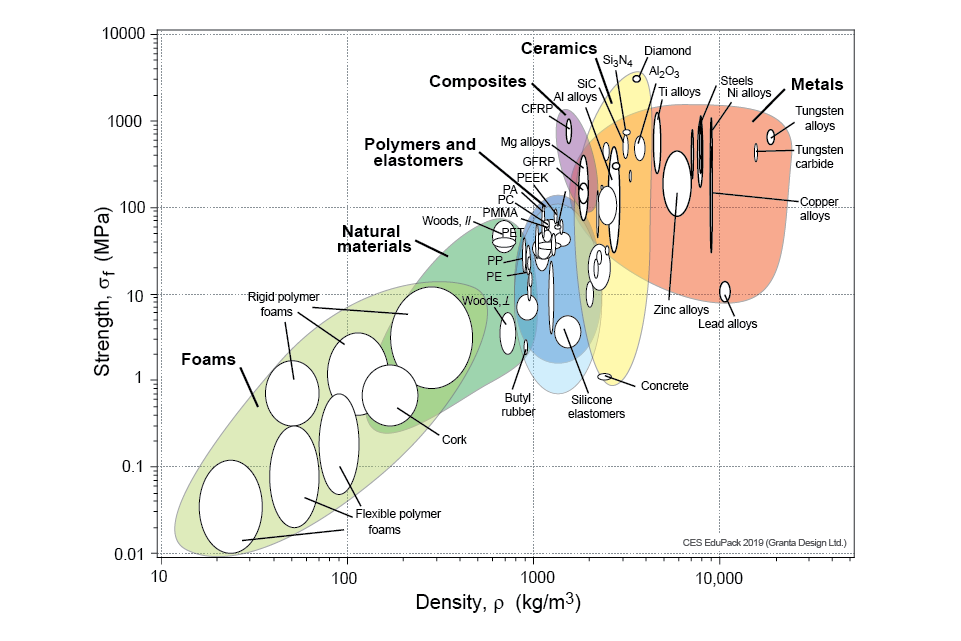
\includegraphics[width=\linewidth]{Photos/strength_density.png}
    \caption{Strength versus Density for Different Materials \cite{ashby}}
    \label{fig:strength_density}
\end{figure}

A hybrid build-up is a method where both metals and composites are used for different structures depending on key factors such as fatigue, damage tolerance, ultimate strength per density ratio, cost of manufacturing, assembly methods, and operational costs. Hybrid designs usually optimized costs and weight of the structure, which results in the wings and stabilizers to be a mainly composite build-up, and the fuselage and other secondary structures to be a metal build-up. Hybrid construction is a newer technology, and as the development of manufacturing of composites advances, this style of construction may become more prevalent in industry. A notable aircraft which uses a hybrid build would be the Boeing 777-X, in which the wings and stabilizers are composite and the fuselage is metallic. The reason the fuselage is metallic and not composite comes down to the difficulties in manufacturing a round and continuous composite structure, such as the fuselage and empennage sections. A notable aircraft which utilizes mainly composite construction is the Boeing 787, see Figure \ref{fig:787 materials}.

\begin{figure}[!h]
    \centering
    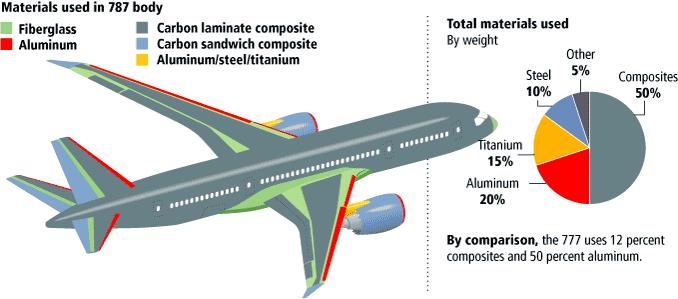
\includegraphics[width=\linewidth]{Photos/787 Materials.png}
    \caption{Material Composition of the B787 \cite{787_Mat}}
    \label{fig:787 materials}
\end{figure}

\FloatBarrier
In Table \ref{tab:pugh_structures}, the benefits and costs for each build-up construction method were weighed in a Pugh matrix given the requirements of cost reduction and the desired aspect ratio and wingspan.

\begin{table}[!h]
\centering
\caption{Pugh Matrix for Structures Material Selection}
\begin{tabular}{|p{3.5cm}||p{3cm}|p{2cm}|p{2cm}|p{2cm}| }
\toprule
\multicolumn{1}{|c||}{\textbf{Criteria}} & \multicolumn{1}{c|}{\textbf{Weight}} &  
\multicolumn{1}{c|}{\textbf{Metallic}} & \multicolumn{1}{c|}{\textbf{Composite}} & \multicolumn{1}{c|}{\textbf{Hybrid}} \\ \hline \hline 
Cost & 10 & 9 & 7 & 8 \\ \hline
Manufacturability & 8 & 8 & 5 & 7 \\  \hline
Strength to Weight & 8 & 7 & 8 & 9 \\  \hline
Fatigue Rating & 5 & 6 & 8 & 7 \\  \hline
Damage Tolerance & 5 & 7 & 6 & 7 \\  \hline
Corrosion Resistance & 4 & 4 & 9 & 8 \\  \hline
Environmental Impact & 3 & 8 & 4 & 6 \\  \hline \hline
 & \textbf{Total} & \textbf{315} & \textbf{292} & \textbf{328} \\
\bottomrule
\end{tabular}
\label{tab:pugh_structures}
\end{table}
\FloatBarrier

Given the Pugh matrix, a hybrid construction is most ideal for the given aircraft requirements. A low fidelity analysis of the structure can assume an isotropic material with the mechanical properties of an ideal composite layup to create a factor to apply to estimations of structure loading given by Raymer \cite{raymer}. A high fidelity analysis of the composite structure would require one of two methods: run FEA on an isotropic material with similar properties to an ideal composite layup, or run FEA with a specific composite build-up in a capable software such as ANSYS.

\subsubsection{Construction and Layout (\textit{CE})}
Given the hybrid construction method, the wings and stabilizers require a newer method of construction compared to the traditional metallic construction. 

Since composite layups are essentially an additive manufacturing technique, the stringers can be integrated into the upper and lower panels of the wings and stabilizers. This alone saves incredible costs and weight by eliminating the use of fasteners in high-load locations. The absence of fasteners increases the damage tolerance and fatigue rating of the structure as well.

Spars are the most important structure to the wings, and arguably the most important on the entire aircraft. These few parts make the entire aircraft fly, and in the process, see a lot of loading cycles over the life of the aircraft. In metal structures, loading cycles cause fatiguing, and then fatigue cracking, which degrades the structure. Traditionally, metallic structures use a 3-piece build-up for the spar: chord on the top and bottom, and a web connecting the two chords. This structure ends-up looking like a C-channel extrusion. The reason the spars are a 3-piece build-up comes down to crack growth and fatigue. A crack starts in the lower chord, but cannot grow through the entire spar since the chord is connected to the web by fasteners. There are a few aircraft that have used a one-piece, or monolithic, metallic spar, some being the Boeing 1-B and the Airbus 320 NEO. There is significant research in learning crack-growth patterns and predicting where cracks will start and grow; opening-up huge possibilities in reducing manufacturing costs by allowing optimized metallic spars to be utilized on low-cost aircraft.

The spars are where composites differ greatly from traditional 3-piece spar construction. Since composite structures do not crack like metal structures when fatigued, a monolithic spar can be utilized. This spar construction reduces costs, but increases the weight due to a thicker layup compared to a simpler 3-piece construction. Due to weight and cost savings, a monolithic composite spar may be the best option. Future work is needed to compare the different spar construction methods.

Ribs in the wings are traditionally multi-piece substructures comprised of machined aluminum parts. The benefit to using aluminum ribs in the wing comes from the fact that composites are difficult to utilize on very complex and dramatic geometry. Due to this fact, a metallic rib layout would minimize costs. In an effort to save more cost and manufacturing troubles, a monolithic rib structure, with the rib posts, chords, webs, and pads machined from a single billet of aluminum, can be investigated. Ribs in the stabilizers are typically not as complex as a rib in the wings due to the lower-loaded structure. In the stabilizers, composite ribs may be utilized for weight savings.

Since the fuselage is a metallic structure, a common layout of frames, stringers, and floor joists can be utilized. The floor joists may be a composite part, as the joists are not primary structure, and the connection method to the frames of the fuselage is by brackets and fasteners. Frames will be dispersed evenly along the length of the fuselage, with several frames being considered "floating", or not connected to the skin of the fuselage, and others being traditional frames. The floating frames are only mounted to the stringers, rather than the actual skin of the fuselage. Floating frames increase fatigue life, as fewer holes are introduced into the fuselage skin.

\subsubsection{Wing Attachment}
There are two primary methods of mating the wings and the fuselage: "bolt-on" or "drop-in". These methods are used equally in industry, as both offer different advantages and carry their own disadvantages. 

A "bolt-on" method essentially bolts the wings onto the fuselage through the wingbox, as the wingbox is integrated into the fuselage. Utilizing shear plates or tension bolts, each wing is attached to the fuselage using fasteners. This method is preferred by most aircraft manufactures, as manufacturing of the fuselage with an integral wingbox and two separate wings is easier to manage in most cases. Using fasteners to attach the wing to the fuselage from the outside poses a difficult engineering challenge which is to make sure load paths are correctly transferring load to the correct primary structures.

The "drop-in" method refers to dropping the fuselage into the space made by the wingbox and wing superstructure. In this method, the wings and wingbox are a singular structure, and the fuselage does not have an integral wingbox. Due to the wings and wingbox being connected before the mating to the fuselage, a more robust connection to the wingbox (internal connection of the spars to the wingbox, rather than fasteners) can be achieved. 

Given that the aircraft is a wide-body, large wingspan structure, a bolt-on method would be preferred, as the manufacturing and logistical challenges in a "drop-in" method are costly.

\subsubsection{Future Work (\textit{CE}}
Future work includes: 

\begin{itemize}
    \item Create a CAD model of the aircraft given the key parameters from the sizing iterations
    \item Create semi-detailed structure in the wing, stabilizers, and fuselage
    \item Complete hand-calculations for basic beam-bending analysis of the wing under flight conditions
    \item Complete higher fidelity FEM analysisof the model, particularly the wing during cruise
\end{itemize}


\subsection{Loads (\textit{MK})}

One important aspect in the structural analysis of the aircraft is determining the limits in the performance of the aircraft. This is specifically done using a V-N diagram, as shown in Figure \ref{figVN}. This diagram incorporates parameters such as wing loading and performance velocities (maneuvering, cruise, and dive velocities) along with limit loading factors. Maximum positive and negative limit loading factors of 3.2 and -1.5 were chosen, respectively, according to the regulations set forth in FAA 14 CFR Part 25.337, Limit Maneuvering Load Factors. These limit loading factors also contain a safety factor of 1.5, as specified in FAA 14 CFR Part 25.303, Factor of Safety. One note about the diagram is that the velocities are displayed as equivalent velocities (KEAS).

\begin{figure}[H]
    \centering
    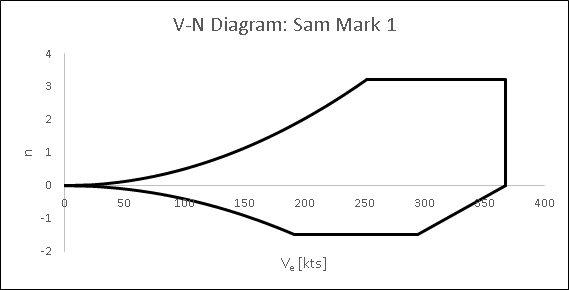
\includegraphics{Photos/VN_Diagram_(2-11-20).png}
    \caption{VN Diagram of Limit Load Factors}
    \label{figVN}
\end{figure}




% \textcolor{red}{
% \begin{itemize}
%     \item Discuss any analysis supporting the sizing analysis.
%     \item Discuss future work.
%     \item AIAA: A V-n diagram for the aircraft with identification of necessary aircraft velocities and design load factors.
%     Required gust loads are specified in 14 Code of Federal Regulations (CFR) Part 25. (This may not come until later)
%     \item AIAA: Materials selection for main structural groups and general structural design, including layout of primary airframe structure as well as the strength capability of the structure
%     and how that compares to what is required at the ultimate load limits of the aircraft.
%     The maximum dive speed of the aircraft shall be specified. (this may not come until later)
% \end{itemize}}